% Drawing 144/01-3 -- folder 144, batch 01, archive page 5 (PDF page 6).
% Transcription: Points $x_0, x_1, gx_0, gx_1, g^2x_0, g^2x_1, \dots, g^{N-1}x_0, g^{N-1}x_1$ et $x_2, gx_2, \dots, g^{N-1}x_2$, disposés en polygones emboîtés qui se resserrent~; une flèche désigne le point central, légendé «~pt fixe par \ill{}~».
% Kind: nested polygons of orbit points. Method 2 (schematic redraw from the facsimile). Status: ok.
% Notes: Redrawn stroke by stroke from the colour scan (250 ppi, rendered at 300 dpi). The polygons are not closed on the page: they are sketched as some twenty separate straight strokes, and each is drawn as it stands, through points placed on its ink (a skeleton follower on the ink served as a local aid). Outer strokes: x_0 -- x_1 -- g x_0 in heavy ink with its three heavy points; a thin stroke from g x_0 to the right, continued by a heavy stroke towards g^2 x_0; the long stroke left of g^2 x_1; the stroke from the top right ending in a heavy dash; the long top stroke; the left-hand stroke. Middle and inner strokes: the stroke round the top from the left; two strokes down the left; the heavy stroke from x_2 towards g^{N-1} x_2; the near-horizontal stroke through the point x_2; the faint stroke from x_2 up to the right; at the right a vertical stroke, two diagonals and a heavy dash. The central point is a heavy blot, and the arrow from the legend « pt fixe par » curves down to it. Labels \small where he wrote them: g^{N-1} x_0, g^{N-1} x_1, x_0, x_1, g x_0, g x_1, g^2 x_0, g^2 x_1, g^{N-1} x_2, x_2, g x_2, and the legend (its last word, illegible in the transcription, left out). Not drawn: the heading M_{g,nu} above the figure, which is text. Overlay check 2026-11-13 (issue 147, Claude Opus 5.5): the redraw, rasterised from its TikZ paths, was laid over the crop; every stroke lies on its ink to within about 0.5 unit and no stroke of the figure is left uncovered. Changed: the two closed polygons of 2026-11-09, whose corners were a reading, are replaced by the strokes of the page. Not compiled (no TeX engine in the session).
% Coordinates: 1 unit = 1 mm = 1/100 of the crop width (bbox in page fractions: [0.17, 0.44, 0.47, 0.59]).
% Redrawn by Claude (claude-opus-5-5), issue #73, 2026-11-09; not checked by a human; not compiled (no TeX in the session).
% Checked by Claude (claude-opus-5-5) 2026-11-13 (issue #147): redrawn stroke by stroke on the 300 dpi colour render of the 250 ppi scan and overlaid; not compiled (no TeX in the session). Not checked by a human. Status: ok.
% Rights: reproduces part of the work -- behind RENDER_TRANSCRIPTS, never published by itself.
\documentclass[tikz,border=3pt]{standalone}
\usepackage{amsmath,amssymb}
\usetikzlibrary{patterns,arrows.meta}
\tikzset{pencil/.style={black!45}, struck/.style={black!35}, mark/.style={circle,draw,inner sep=1.3pt}, pt/.style={circle,fill,inner sep=0.9pt}, opt/.style={circle,draw,fill=white,inner sep=1.1pt}}
\begin{document}
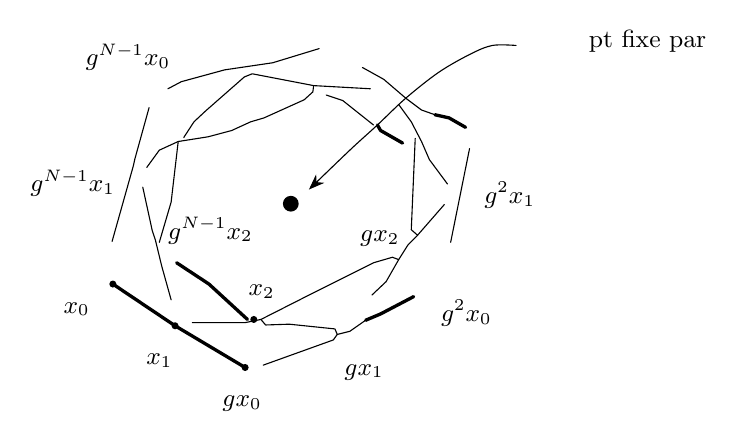
\begin{tikzpicture}[x=1mm,y=1mm,line cap=round,line join=round,font=\scriptsize]
\draw[very thick] (12.1,-44.8) -- (20,-50.1) -- (28.9,-55.4);
\draw (31.2,-55.1) -- (40.1,-51.9) -- (40.6,-51.2);
\draw (40.6,-51.2) -- (42.2,-50.8) -- (44.2,-49.4);
\draw[very thick] (44.2,-49.4) -- (46.1,-48.6) -- (50.3,-46.4);
\draw (55,-39.5) -- (57.4,-27.6);
\draw (43.8,-17.3) -- (46.5,-18.8) -- (49.3,-21.2) -- (51.3,-22.7) -- (53,-23.3);
\draw[very thick] (53,-23.3) -- (54.8,-23.7) -- (56.9,-24.9);
\draw (19.1,-20) -- (20.8,-19.1) -- (26.3,-17.6) -- (32.4,-16.7) -- (38.3,-14.9);
\draw (16.7,-22.4) -- (14.9,-28.9) -- (14.7,-29.8) -- (12,-39.4);
\draw (21.1,-26.2) -- (22.4,-24.2) -- (23.9,-22.8) -- (28.8,-18.5) -- (29.8,-18.1) -- (37.6,-19.6) -- (44.8,-20);
\draw (39.2,-20.8) -- (41.3,-21.5) -- (45.2,-24.6);
\draw[very thick] (45.7,-24.6) -- (46.1,-25.3) -- (48.9,-26.9);
\draw (48.4,-22) -- (50,-24.2) -- (51.3,-26.7) -- (52.3,-29) -- (54.6,-32.1);
\draw (50.5,-26.3) -- (50,-37.9) -- (50.8,-38.6);
\draw (54.2,-34.7) -- (50.8,-38.6) -- (49.6,-39.8) -- (48.4,-41.7) -- (46.8,-44.5) -- (45,-46.2);
\draw (30.9,-49.3) -- (38,-45.7) -- (45.2,-42.1) -- (47.6,-41.4) -- (48.4,-41.7);
\draw[very thick] (29.2,-49.3) -- (24.3,-44.8) -- (20.2,-42.1);
\draw (22.2,-49.7) -- (28.9,-49.7) -- (30.9,-49.3) -- (31.5,-50) -- (34.5,-49.9) -- (40.3,-50.5) -- (40.6,-51.2);
\draw (16.4,-30) -- (18,-27.8) -- (20.4,-26.7) -- (24.2,-26.1) -- (27.2,-25.3) -- (29.6,-24.2) -- (31.3,-23.7) -- (36.4,-21.4) -- (37.5,-20.4) -- (37.6,-19.6);
\draw (20.4,-26.7) -- (19.5,-34.4) -- (18,-39.5);
\draw (15.9,-32.5) -- (17.1,-38) -- (17.5,-39.2) -- (18.3,-42.5) -- (19.5,-46.8);
\draw[-{Stealth[length=2mm]}] plot[smooth, tension=0.55] coordinates {(63.3,-14.5) (60.3,-14.5) (57.5,-15.6) (53.5,-17.9) (49.3,-21.2) (45.7,-24.6) (42.3,-27.7) (37,-32.8)};
\node[pt] at (12.1,-44.8) {};
\node[pt] at (20,-50.1) {};
\node[pt] at (28.9,-55.4) {};
\node[pt] at (30,-49.3) {};
\fill (34.7,-34.6) circle[radius=1];
\node[inner sep=1pt] at (80,-14) {\small pt fixe par};
\node[inner sep=1pt] at (14,-16) {\small $g^{N-1}x_0$};
\node[inner sep=1pt] at (7,-32) {\small $g^{N-1}x_1$};
\node[inner sep=1pt] at (7.5,-48) {\small $x_0$};
\node[inner sep=1pt] at (18,-54.5) {\small $x_1$};
\node[inner sep=1pt] at (28.5,-60) {\small $gx_0$};
\node[inner sep=1pt] at (44,-56) {\small $gx_1$};
\node[inner sep=1pt] at (57,-48.5) {\small $g^2x_0$};
\node[inner sep=1pt] at (62.5,-33.5) {\small $g^2x_1$};
\node[inner sep=1pt] at (24.5,-38) {\small $g^{N-1}x_2$};
\node[inner sep=1pt] at (31,-45.8) {\small $x_2$};
\node[inner sep=1pt] at (46,-39) {\small $gx_2$};
\end{tikzpicture}
\end{document}
